\documentclass{article}
\usepackage{multicol}
\usepackage{lipsum}
\usepackage{lineno}
\usepackage{parskip}
\usepackage{graphicx}

\title{%
Chop Chop \\
  \large Group Report}
\author{
  Connor, Wood\\
  \texttt{cw668}
  \and
  Will, Haysom\\
  \texttt{wah20}
  \and
  Dean, Gooding\\
  \texttt{Dmag2}
  \and
  Beth, Hill\\
  \texttt{Berh2}
  \and
  Jack, Fermer\\
  \texttt{Jdf50}
}

\begin{document}

\maketitle

\pagebreak

\pagenumbering{roman}
\linenumbers

\begin{abstract}
  \addcontentsline{toc}{section}{Abstract}
      This report surrounds our group software development project, a smart cooking assistant called \emph{Chop Chop}. 
    
      In this report we will showcase our group project. We will be evaluating not only the software we made but also how we made it, looking into our design, development, and ways of working. In addition to this, we will 
  \end{abstract}

  \pagebreak

  \tableofcontents

  \pagebreak

  \pagenumbering{arabic}

  %\begin{multicols}{2}

    \section{Introduction}
Chop Chop makes cooking more accessible by offering hands-free, smart recipes. Our smart recipes allow users to get on with cooking without having to worry about looking through the steps of a recipe, scrolling a screen with messy hands, or starting timers. It achieves this by using artificial intelligence, computer vision, and a full-stack application.

    \section{Research}
    \subsection{Object detection}
    Our project's flagship feature was our custom real-time object detection system. This would be used to detect culinary objects such as food and utensils which would dictate when a recipe step had been completed.
    
None of us on the project had experience creating an object detection system. So, we began by doing some research. 

With the huge demand for real-time object detection in the modern age many different algorithms have emerged.

Faster R-CNN offers a real-time object detection algorithm version of R-CNN. “One of the most accurate object detection algorithms” \cite{FasterRCNN} with the drawback of “requires a lot of power at inference time” IE when running in real-time. So, detecting small food objects in a kitchen would be perfect. However, we hoped to run on a Raspberry Pi (a hub in the kitchen area), and we fear the Raspberry Pi will not have the computational power required \cite{Fast-CNN-Rasberry-Pi} at inference time.

Detectron2- Created by Facebook AI research it claims to “provides state-of-the-art detection and segmentation algorithms” \cite{wu2019detectron2} and has been used in many Facebook products such as “Smart Camera for new Portal video-calling devices” \cite{metasmartcameras}. It’s built using the COCO, LVIS, CityScape, and VOC20 datasets, this creates an accurate dataset with an MNAP. However, in many cases “YOLOv8 models outperformed the detectron2 mode” \cite{ai5010005}.

YOLO – You Only Look Once, “It is a state-of-the-art, real-time object detection system which offers extreme levels of speed and accuracy.” \cite{rajeshwari2019object}, that is around “1000x faster than RCNN and 100x faster than the Fast R-CNN model” \cite{rajeshwari2019object}.  It's also shown to have a much higher mAP50-95 "96.7\%" compared to detectron2 (Faster RCNN-101) at "83.554\%"  "YOLO proves to be a cleaner and more efficient" \cite{joiya2022object}, which gave us more confidence if we do eventually choose to run it on slower hardware such as a Raspberry Pi.

Dean reached out to an ex-colleague who had experience in this area. They suggested using YOLOv8 \cite{Jocher_Ultralytics_YOLO_2023} as a base for real-time object detection and suggested using Roboflow \cite{RoboFlow-Software} for dataset management. 

RoboFlow \cite{RoboFlow-Software} is a site where you can easily collaboratively create image datasets. It allows you to upload images you have taken for training, delegate annotation jobs out to different members of the team, and then create a dataset which can be downloaded and trained locally. It was one of the few sites that offered an immense data set (max 10,000 images) with an easy-to-use interface, all for free.

During our research process, we tried out Roboflow and used a trial of their training cloud computers. With only 100 images we were able to confidently detect a Rubik's cube, being held, rotated in the hand, and placed under different backgrounds. Given the lack of experience we had, the relatively small number of images, and the very accurate results we achieved. We were confident that scaling up to whole recipes should on paper be very possible.

    \section{Aims}

    \section{Ways of Working}
    \subsection{Source Control}
    One of the key components to Chop-Chops’ success was our well-set-up and organised GitLab repository. 

    Initially, we decided to create a Gantt chart to record the project timeline and delegate deliverables, which was broken down into two-week sprints. Once all members approved this, it was sent to our supervisor who provided insight into improvements to ensure the project worked effectively. An example of this would be adding our module assessments to the chart to accurately manage and consider our university commitments and workload. 

    A scrum-style agile approach was adopted to our project management strategy. We broke down our Gantt charts’ deliverables into “Issues” on Gitlab. Issues were put on our virtual board, which had four categories, Open, In Development, Review/ Testing, and Closed. These issues were assigned and then moved across given their completion state. 

    From our team’s year-in-industry experience, we adopted a review before merging convention. This rule ensures that tasks were overlooked by other members before being added to the main branch from their working one. This had two main advantages. One was a hugely reduced chance of buggy code getting into the main branch. Two: you gained knowledge of how the rest of the project worked outside of your assigned issues. To enforce this, we locked the main branch from being merged and required at least one approval before the merge.

    We aimed to ensure the main branch was kept as clean as possible; we were mindful of what should and should not be on the repo. This included adding rules to the git ignore file when needed, pruning unnecessary files, and ensuring consistency in naming conventions for files and folders.

    \subsection{Meetings}
    \subsubsection{Meeting Documents}
    During our sprints, we scheduled one team meeting and one supervisor meeting each week. Ideally, we arranged the supervisor meeting to take place after the team meeting, allowing us to bring any discussions raised in the team meeting to the supervisor within the same week.
    Throughout the week a shared team document was available for any members to note down any questions or issues that they wanted to raise in the team meeting. This functioned very well as it meant discussions were not accidentally overlooked during the meeting and it also allowed other members to see the discussions points raised and prepare prior to the meeting.
    We also made use of the GitLabs issues board and our own Gannt chart to keep ourselves on schedule throughout the project. These tools allowed us to easily check what work was still outstanding for the week and compare the progress we were making to our initials estimates when starting out. As this was a particularly large project to undertake it was crucial we kept ourselves on track this way.
    \subsubsection{Team Meetings}
    At the beginning of each team meeting, we allocated a minute-taker to record the discussions. We would then begin by addressing any discussion points or questions raised in the shared document or brought up by members during the meeting. The practice of having discussions pre-documented in the shared file significantly sped up the note-taking process, enabling us to focus more on the discussions themselves. 
    Following the discussions, we would quickly cover all issues closed on the GitLabs since last meeting, making note of them in the minutes, before reviewing any outstanding issues. We made sure that each team member individually was making good progress and was clear with what work was still to be done and provided team assistance to any members that were encountering any difficulties with their work.
    Finally, we would create new issues aligned with the progress steps outlined on the Gannt Chart and assign them out to team members based on their current workloads and experience in the given areas of the project.
    \subsubsection{Supervisor Meetings}
    Our supervisor meetings were usually well organised as we would make notes during the team meetings for any discussions to be bought up to the supervisor. Any feedback or recommendations were then considered, and issues and objectives updated to reflect any changes from the meeting.
    As well as this, we made sure to keep our supervisor updated on our progress and any issues closed since the last meeting and inform them of the issues outstanding and assigned for this week. This way we made sure the supervisor was always aware of the work we were aiming to achieve for next week and could hold us accountable for any delays.


    \section{Design}
    \subsection{Frontend}
    Figma was the main tool which we used to craft the frontend design of our web application. We were able to create and pull ideas from each other and prototype how we wanted the design of the application to look by using its collaborative interface. Within this section, we outline our process of exploring and integrating various ideas into our designs, as well as how we utilised Figma to translate these designs into functional code.

    \subsubsection{Research}
    
    Our design process began by investigating and researching what other recipe applications offered in terms of layout, features, and user experience. The three main recipe applications which we focused our research on was BBC Good Foods, AllRecipes and Yummly. 
    
    \paragraph{Featured Recipe}
    Our findings found that the majority of the sites that we looked at showed a featured article or recipe which was the the forefront of the homepage. This component would usually include a background image, title, description, and a button directing users to the featured collection. We quite liked this idea, as it was visually appealing, and an effective way to draw users attention to a focal point on the homepage. We also liked how it could streamline user navigation, and that we could implement our own functionality to make the component work well with our application.
    
    \begin{figure}[htbp]
      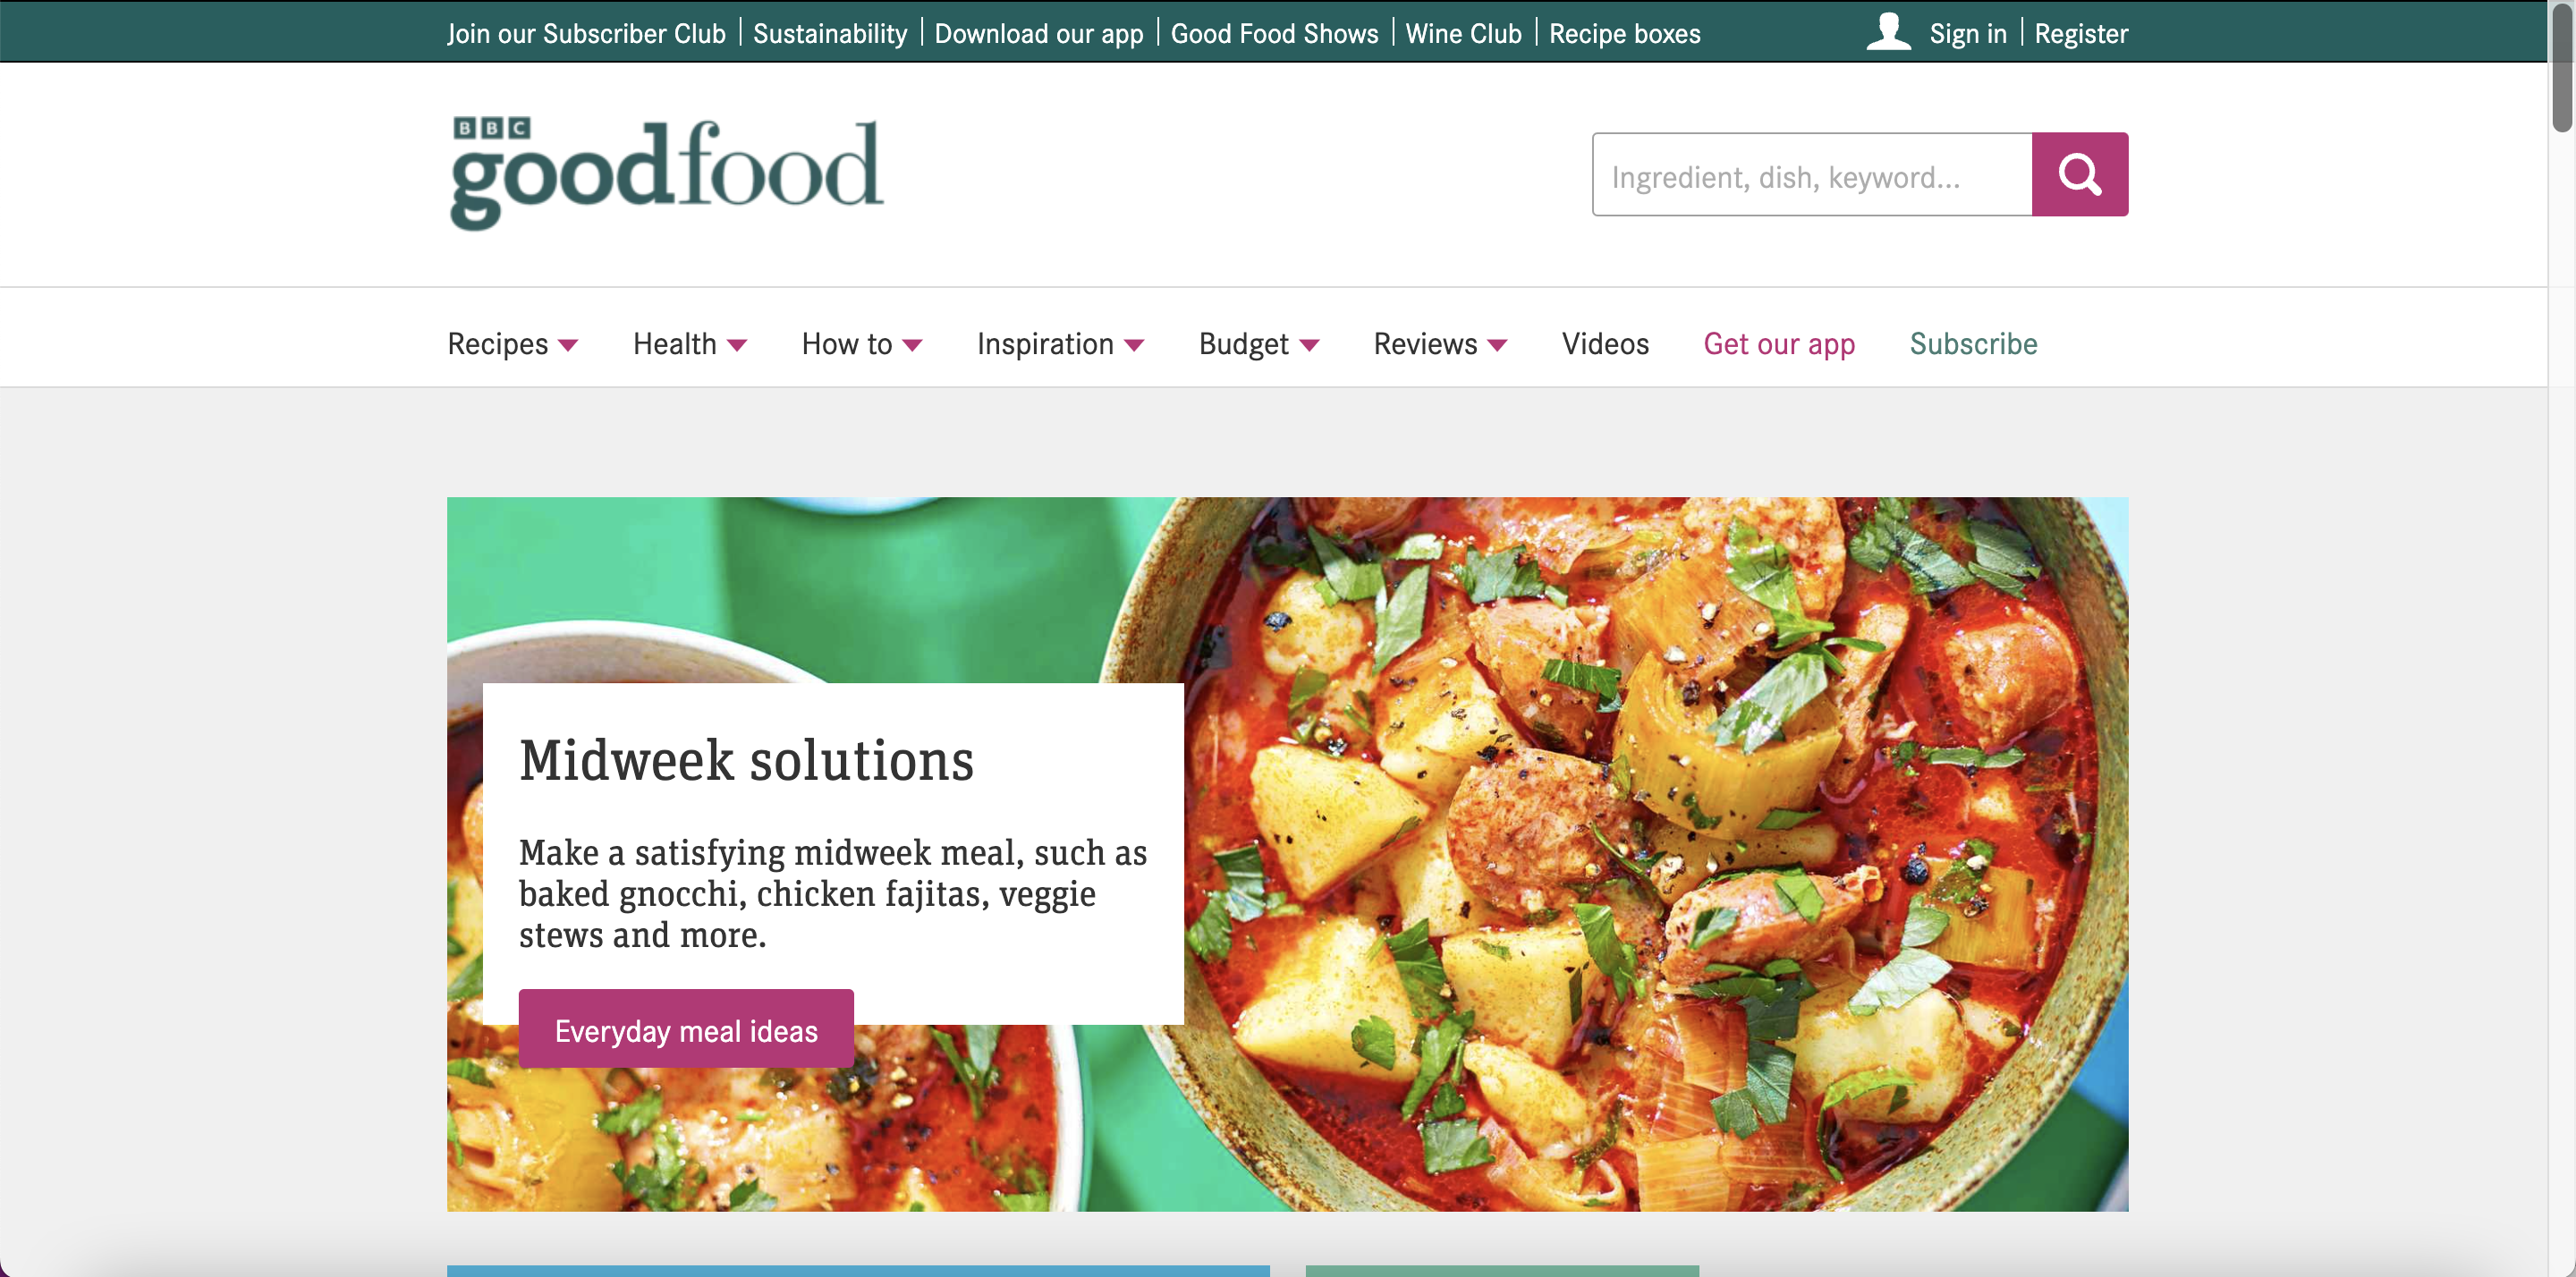
\includegraphics[width=1.0\textwidth]{BBCGF featured-image.png}
      \centering
      \caption{insert caption here}
    \end{figure}

    \paragraph{Recipe cards}
    Each site also used cards as a way to display each recipe. We found that this was an effective way to display each of the recipes, while only showing the necessary information needed for the user.
    
    On Yummly, a variation of their recipe cards caught our attention with an interactive hover feature. Initially displaying just the recipe title, hovering over the card revealed more details about the recipe. We aimed to incorporate a similar functionality into our own cards.
    
    \begin{figure}[htbp]
      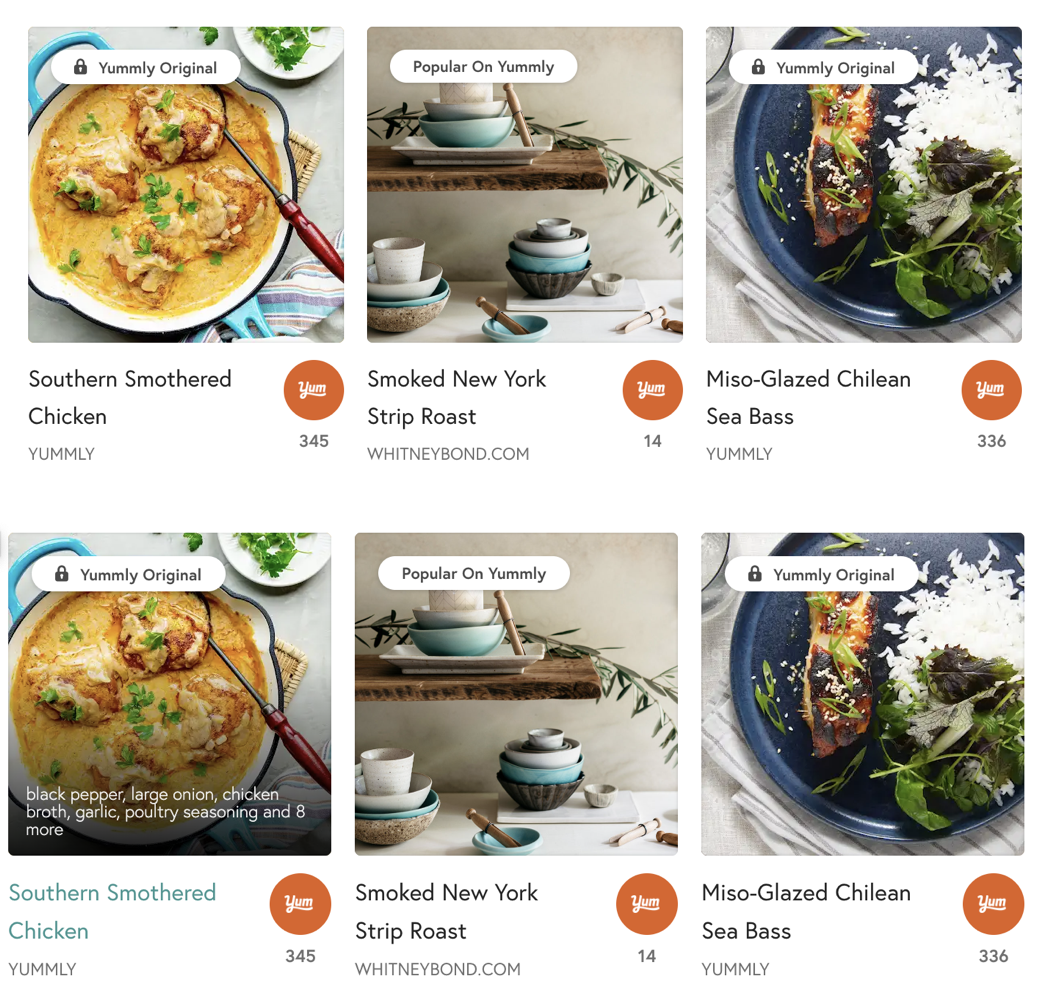
\includegraphics[width=1.0\textwidth]{Yummly recipe cards.png}
      \centering
      \caption{insert caption here}
    \end{figure}

    \paragraph{Recipe Overview}
    For the Recipe Overview page, we wanted the user to be able to see a summary of the recipe and navigate between seeing the recipe steps and the ingredients in a seamless way.
    
    To keep the design of the page simple and clean, we split the page into two sections: the header and the information. The header of the page would show off important information about the recipe, such as the name, a description and a summary of how long the recipe will take to prepare. This section would also feature a start recipe button to take the user to the recipe carousel page.
    
    The information section of the page would showcase both the ingredients and recipe portions of the overview.
    
    After looking at the 3 initial sites, we discovered that the layout was overly cluttered, and the transition between viewing the recipe and its ingredients was not seamless. Instead, most sites placed the ingredients and recipe either side by side or one after the other, which disrupted the flow of navigation.
    
    Instead, we opted for a switcher component that enables users to toggle between viewing the recipe and the ingredients. We believed that this approach would reduce clutter on the page and separate information in a more organised manner. We found inspiration for this functionality on W3Schools.
    
    \begin{figure}[htbp]
      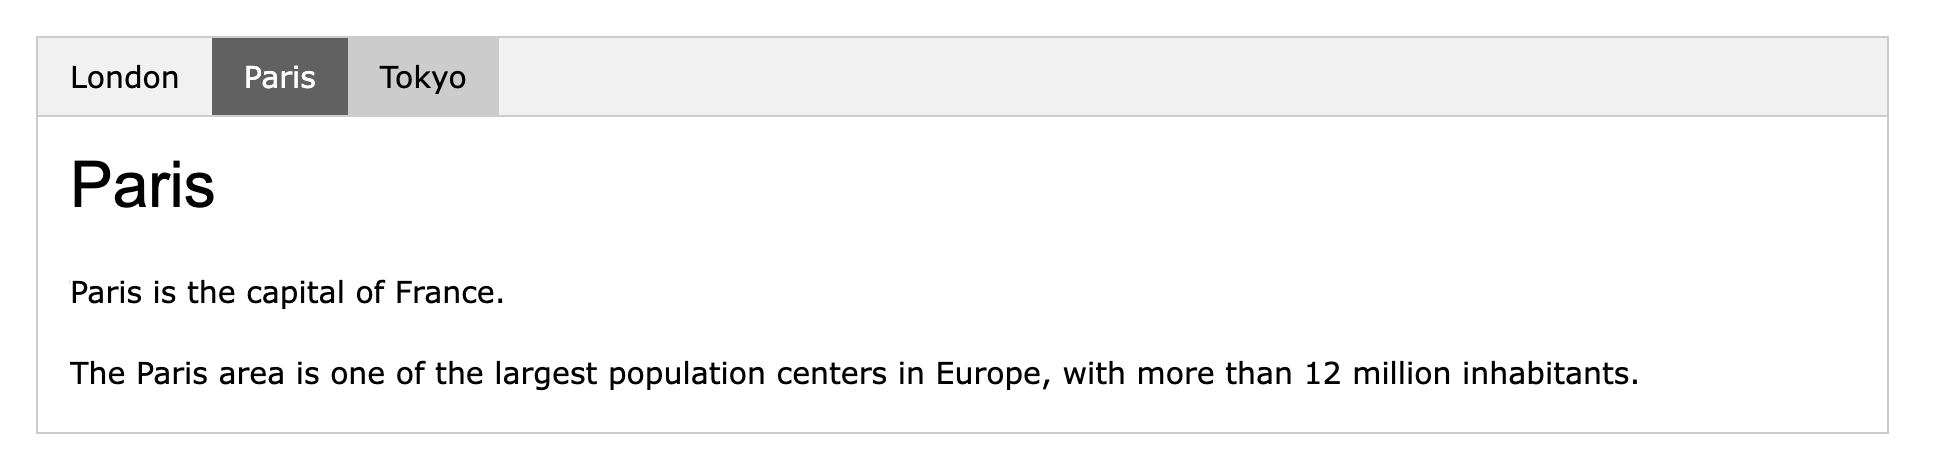
\includegraphics[width=1.0\textwidth]{W3Schools tabbed component.png}
      \centering
      \caption{insert caption here}
    \end{figure}

    We liked the simplicity of this design and the effective functionality to show off information without cluttering the page. 

    \paragraph{Colour Palette}
    To begin our investigation into which colour palette should be used for the frontend, we decided to investigate any accessibility issues which we will have to take in to consideration to ensure that our design enhanced readability and usability for all users. 

    During this investigation, we found that the use of bright colours may cause pain for those who suffer with low vision or dyslexia, and may also prevent them from being able to read information from the page. This means that websites need to have a low brightness background to accommodate for this disability.
    
    Users also need a high contrast between the text and the background on a page. According to the W3C accessibility standards, people will be able to read information better on a page which incorporates dark text on a light background. We wanted to select colours for our frontend which would meet both of these accessibility criteria and found that a neutral tone for our main colour scheme would effectively meet these standards.
    
    For the background of the the web application, we opted to use a pale peach colour. We selected this colour as it would provide a warmth to the page while also ensuring that users who struggle with bright backgrounds are not overwhelmed when reading information. Furthermore, the selection of this colour made it easier to find secondary colours for text and highlights that would provide a bold contrast.

    Following our research from the initial recipe websites, we noted that both BBC Good Foods and Yummly incorporated green into their website design. We liked the use of the colour green since it is associated with promoting healthy eating, and although our application is not necessarily for this purpose, it can make people feel better about what they eat.

    We also found that this colour contrasts well with the pale peach background and is not harsh on the eyes, providing a bold contrast to increase readability for users.

    \subsubsection{Figma vs Zeplin}
    Before we began to design the prototype of the frontend, we had to decide which software application we should use. From prior experience during our placement year, we initially chose to use either Figma or Zeplin.

    Within our research, we found that Zeplin is primarily a collaboration and handoff tool whereas Figma is a comprehensive design tool that enables collaborative design, prototyping, and sharing within a single platform. This means that you could create designs directly using Figma, while on Zeplin, designs must be created using a dedicated design tool such as Sketch or Adobe XD, and then imported. 
    
    Figma also features a Dev Mode interface that allows for developers to translate created designs into code more efficiently. As a team, we liked the use of this feature since we would be able to streamline the design-to-development workflow and reduce the use of repetitive, manual coding.
    
    While Zeplin does also feature some developer tools, Figma is exclusively tailored for the design process. This means that Figma can provide a better experience while designing prototypes as it doe not have the additional complexity of features which are shown within Zeplin. 

    After considering the pros and cons of both applications, combined with the research which we conducted, we decided that Figma would be the best solution for us.
    
    \subsubsection{Designs: Version 1}
    The initial iteration of the designs prioritised the application's functionality over user experience considerations. We used our prior research to design a homepage which would allow the user to view and navigate to recipes easily as well as providing essential information to the user. 

    Inspired by our research, we designed our own featured recipe component, recipe cards and recipe pages. 

    \subsubsection{Designs: Version 2}

    \subsection{Architecture}
  

    \section{Development}
    \subsection{Backend}
        The backend is divided into several sections: API, controller, interpreter, and object detection. Additionally, we have utilities and tests, which support and are utilised within other sections. The backend is initiated from 'main.py', which launches the controller, API, and our logging system, producing two separate log files: one called 'detection' and one called 'API' to help us track the status of the program. We also have 'config.py', which houses common variables used throughout the backend. This allows us to easily change any of these variables without delving too deeply into the backend.
    \subsubsection{Controller}
    Our controller keeps state for the backend: storing the current recipe and step, taking messages from the API to the database, and handling detection events from the interpreter. It is built from 3 core scripts, the Controller main script, a manageThread script and a recipe script. 
    The recipe script is for all the getter and setter functions that are recipe dependent. This includes functions such as get\textunderscore command\textunderscore for\textunderscore step to be able to read and serve the human readable commands to the frontend and get\textunderscore progression\textunderscore requirements\textunderscore for\textunderscore step to get and serve the progression objects to the interpreter. We split these functions into a separate script from the main Controller as they are recipe dependent, meaning we need to have already selected a recipe in the initialisation stage of this script and we wanted to keep this function out of the main controller script as that also houses recipe independent functions.
    The main Controller script contains functions for starting new recipes, recipe dependent functions called from the recipes script and recipe independent functions such as retrieving all recipe metadata for displaying multiple recipes on the frontend.
    \subsubsection{Interpreter}
    \subsubsection{API}
    \subsection{Frontend}
 
    \subsection{Database}
    \subsubsection{JSON}
    We originally built a JSON database to quickly get started with storing recipes. We broke the initial database into separate recipes, each with three distinct areas. Recipe Details contained the recipe ID, Name and Description, Recipe Ingredients contained all the ingredient Names as well as Amount and Unit. Recipe Steps then contained Steps in human readable form, the Progression Object and Inhibitor for the backends understanding and the Camera which the step is expected to be completed under.
    We chose to use JSON to start with due to its quick and simple nature to set up, allowing us to quickly begin testing the process of displaying recipe details and ingredients on the frontend and progressing through recipe steps with the backend.
    When breaking the recipes into separate steps we knew we had to do it in a way that could be easily translated into Progression Objects and Inhibitor Objects. From our first database we had the steps broken down into their most simple form so that the neural network would only ever have one object to be looking for at once. It was important that this step was done early as it led the way for knowing what images we would need to have for our training dataset.
    \subsubsection{SQL}
    Further into the project, once we had a good setup for displaying and progressing our recipes, we wanted to add a significant amount of “dummy data” to fill out the frontend application and allow for features such as featured recipes and recipe searching. It became clear that the JSON database would no longer be the best way to store our recipes and we instead opted to transition to an SQL database before progressing with adding the additional recipes and search functionality.
    After deciding to migrate to an SQL database, we conducted research and opted for SQLite over other SQL database engines. This choice stemmed from our desire for a straightforward implementation while still leveraging the features of SQL and not needing to start running any more servers which would have been required for an SQL server.
    The SQL database comprises five tables, three of these tables are mapped from the same segments that were split from the JSON data. These tables include Recipes, which store core recipe information such as name and description, Steps which is linked to recipes in a one-to-many relationship, and Ingredients, also linked to recipes in a one-to-many relationship. Recipes contains the same information as it did in the JSON, while Steps and Ingredients needed a column added for RecipeID to now be able to link it back to the recipe they belong to.
    Additionally, the database includes two new tables to accommodate the work done with voices. The Voices table assigns a unique ID to each voice, and the Recipe\textunderscore Voices table facilitates many-to-many connections between recipes and voice recordings.
    \subsubsection{Multimedia Gallery}
    As well as the SQL database the final project also contains a file storage server to store our photos and voice recordings for recipe steps. This is local file storage server with its location stored inside the SQL database.
    This file storage is called using a custom HTML web request to retrieve the images and voice recordings. We chose to store our recipe images like this as we found it to be the simplest and easiest way to store photos with a focus on scalability.

    \subsection{Data Collection \& Training}
    \subsubsection{RoboFlow}
    For developing our object detection system, we needed a trained model. From our research, we decided to use Roboflow for data collection and management and trained with YOLOv8.
    
To train, we first needed to collect many images of the object we wanted to detect. We found during development that it is best to start with lots of good-quality images of the object; They should be in good lighting and well-framed. Then many different positions of objects in the frame. Finally, gathering some more obscure images. These can be in different lighting conditions, from far away, and with multiple other objects in the frame as well. These all create a diverse data set, which increases the chance of detection.

Once a significant number of images had been gathered (around 100) they were uploaded to Roboflow for annotating. Annotation jobs can be generated and sent to each person on the project. We decided to use box annotation, as it was significantly quicker to annotate and in our preliminary tests offered the same level of object detection that poly-selection did.

Each annotation was then reviewed by someone else before being added to the dataset. This ensured that the dataset was accurate in its annotations as small mistakes could teach the AI the wrong classification.

When all images are annotated a new YOLOv8 dataset can be generated. Before this Roboflow will split up your images into training, testing, and validation. Training will teach AI, validation are used to as it trains test how good the AI is getting. Testing “a test data set is a separate sample, an unseen data set, to provide an unbiased final evaluation of a model fit.” \cite{trainvalidtest} It will resize the image to 640x640 which greatly reduces training time, and smaller images reduce computational cost. 

Finally, it generates extra images through augmentation. We chose Shear ±15° and Brightness ±25\%. Shear would simulate different camera angles, which would provide greater angle coverage. Brightness would widen the number of handled lighting conditions, as different kitchens could have very varied levels of brightness.

    \subsubsection{Training with CUDA}
    While RoboFlow did offer the option to train the models for us, it required monetary payments, so we opted to train on our Nivida GPU using CUDA \cite{cudacuda}.
    ...... HERE

    \subsubsection{Reviewing \& Improving}


    \section{Testing}

    \section{Results}

    \section{Future Work}

    \section{Conclusion}

    \pagebreak

    
  %\end{multicols}
  
  \addcontentsline{toc}{section}{References}

  \bibliographystyle{ieeetr}
  
  \bibliography{group-doc}

\end{document}